\section{Testbench}

For testbenches, I used \texttt{cocotb} to write Python scripts that will interface with \texttt{iverilog} for simulation.
Initially, I used module-level testbenches to verify the functionality of individual components.
Then, I created an integrated testbench to test the entire RISC-V processor with a simple assembly programs written in the RV32I set.

\subsection{Module-Level Testbenches}

\begin{minted}[fontsize=\small,linenos]{python}
import cocotb
from cocotb.triggers import Timer

@cocotb.test()
async def test_u_imm(dut):
    dut.instr.value = 0b00000000000000001110000010110111  # lui x1, 14
    imm_ext = 0b00000000000000001110000000000000  # {instr[31:12], {12{'0}}}
    await Timer(1, units="ns")
    assert dut.imm_ext.value == imm_ext
\end{minted}

\begin{figure}[H]
    \centering
    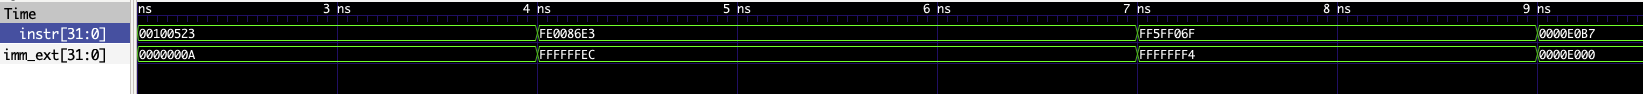
\includegraphics[width=\textwidth]{media/imm_ext_waveform}
    \caption{Waveform of the immediate extender testbench. The first value maps to the code snippet above, and the rest tests the other immediate types.}
    \label{fig:imm-extender}
\end{figure}

The above code is an example of a module-level testbench for the immediate extender module.
It simply injects an I-type instruction (\texttt{lui x1, 14}) into \texttt{dut} (immediate extender) checks if it produces the expected immediate value.
The results are shown in Figure~\ref{fig:imm-extender}.
Similarly, I wrote testbenches for other modules to verify their functionality independent of the CPU.

\subsection{Integrated Testbench}

\begin{minted}[fontsize=\small,linenos,frame=lines,framesep=2mm]{python}
import cocotb
from cocotb.triggers import ClockCycles
from utils import (
    init_clock,
    write_program_to_memory,
    reset_risc_v,
    get_register_value,
)
from functools import partial

@cocotb.test()
async def test_integer_register_immediate(dut):
    """
    Test integer register-immediate instructions (I-type).

    addi x1, x0, 0x80F    # pc = 0x00, x1 = 0xFFFF_F80F = -2033
    slti x2, x1, -2032    # pc = 0x04, x2 = 0x00000001; x1 < -2032
    sltiu x3, x1, 10   # pc = 0x08, x3 = 0x00000000; x1 > 10 (unsigned)
    sltiu x4, x0, 1      # pc = 0x0C, x4 = 0x00000001; x0 < 0x0000_0001 (unsigned) -- only possible when rs1 is 0
    andi x5, x1, 0x0FF    # pc = 0x10, x5 = 0x0000_000F
    ori x6, x5, 0xFCF    # pc = 0x14, x6 = 0xFFFF_FFCF
    xori x7, x6, 0xFF0    # pc = 0x18, x7 = 0x0000_003F
    xori x8, x6, -1      # pc = 0x1C, x8 = 0x0000_0030
    slli x9, x7, 24       # pc = 0x1C, x9 = 0x3F00_0000
    srli x10, x9, 2       # pc = 0x20, x10 = 0x0FC0_0000
    srai x11, x10, 2      # pc = 0x24, x11 = 0x003F_0000
    """
    registers = partial(get_register_value, dut.u_risc_v.u_register_file)
    init_clock(dut)
    reset_risc_v(dut.u_risc_v)
    data = [
        0x80F00093,  # addi x1 x0 -2033
        0x8100A113,  # slti x2 x1 -2032
        0x00A0B193,  # sltiu x3 x1 10
        0x00103213,  # sltiu x4 x0 1
        0x0FF0F293,  # andi x5 x1 255
        0xFCF2E313,  # ori x6 x5 -49
        0xFF034393,  # xori x7 x6 -16
        0xFFF34413,  # xori x8 x6 -1
        0x01839493,  # slli x9 x7 24
        0x0024D513,  # srli x10 x9 2
        0x40255593,  # srai x11 x10 2
    ]
    write_program_to_memory(dut.u_memory, data)
    await ClockCycles(dut.clk, 2)

    await ClockCycles(dut.clk, 22)  # 11 instructions, 2 cycles each
    assert registers(1) == 0xFFFFF80F
    assert registers(2) == 0x00000001
    assert registers(3) == 0x00000000
    assert registers(4) == 0x00000001
    assert registers(5) == 0x0000000F
    assert registers(6) == 0xFFFFFFCF
    assert registers(7) == 0x0000003F
    assert registers(8) == 0x00000030
    assert registers(9) == 0x3F000000
    assert registers(10) == 0x0FC00000
    assert registers(11) == 0x03F00000
\end{minted}

\begin{figure}[H]
    \centering
    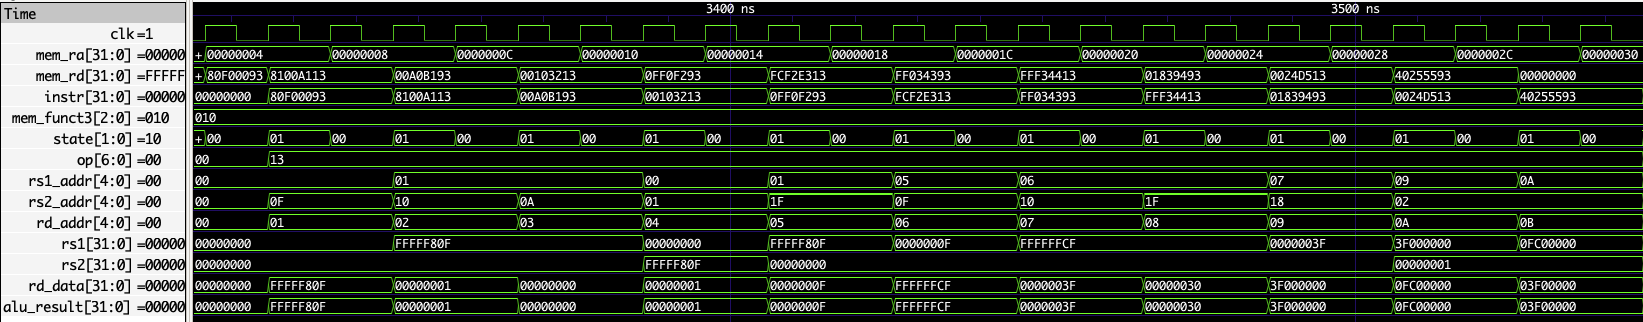
\includegraphics[width=\textwidth]{media/int_i_type_waveform}
    \caption{Waveform of the testbench for I-type instructions. The destination register data matches the expected values for each instruction.}
    \label{fig:i-type-waveform}
\end{figure}

Above is an example of an integrated testbench for the RISC-V processor.
The \texttt{dut} object represents the top-level module of the RISC-V processor, which includes the core and memory module.
Each tested instruction targets integer operation of I-type instructions, including immediate arithmetic operations and logical operations.
These instructions are manually encoded into machine code and loaded into the memory model connected to the RISC-V processor.
The test runs the simulation for 22 clock cycles (since the target instructions take 2 cycles each) and checks the values of registers \texttt{x1} through \texttt{x11} to ensure that each instruction executed as expected.
Refer to Figure~\ref{fig:i-type-waveform} for the waveform of the testbench.

\begin{minted}[fontsize=\small,linenos,frame=lines,framesep=2mm]{asm}
lui x1, 0xFEDCC         # pc = 0x00, x1 = 0xFEDCC000
addi x1, x1, 0xA98      # pc = 0x04, x1 = 0xFEDCBA98
srli x2, x1, 4          # pc = 0x08, x2 = 0x0FEDCBA9
srai x3, x1, 4          # pc = 0x0C, x3 = 0xFFEDCBA9
xori x4, x3, -1         # pc = 0x10, x4 = 0x00123456
addi x5, x0, 2          # pc = 0x14, x5 = 0x00000002
add x6, x5, x4          # pc = 0x18, x6 = 0x00123458
sub x7, x6, x4          # pc = 0x1C, x7 = 0x00000002
sll x8, x4, x5          # pc = 0x20, x8 = 0x0048D158
ori x9, x8, 7           # pc = 0x24, x9 = 0x0048D15F
auipc x10, 0x12345      # pc = 0x28, x10 = 0x12345028
sw x1, 98(x5)           # pc = 0x2C, mem[0x00000002 + 98] = 0xFEDCBA98
lw x11, 98(x5)          # pc = 0x30, x11 = 0xFEDCBA98
\end{minted}

\begin{figure}[H]
    \centering
    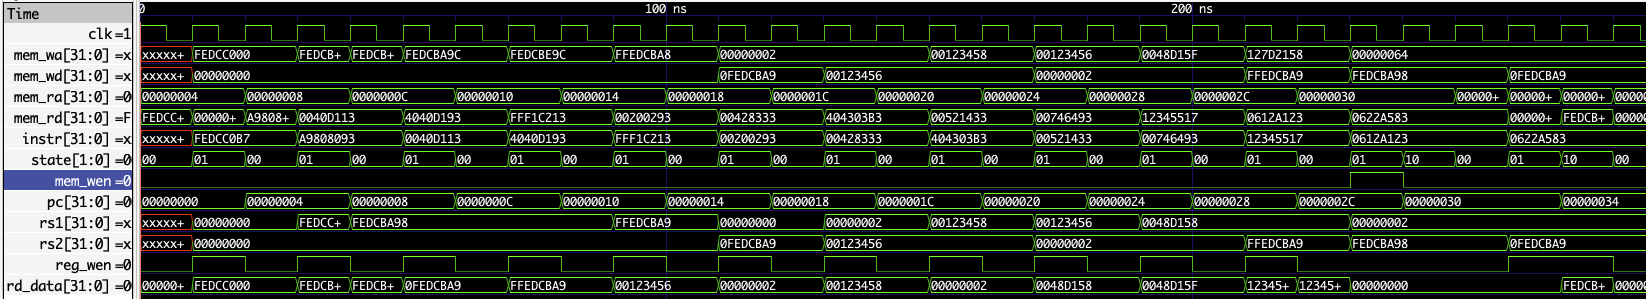
\includegraphics[width=\textwidth]{media/r_i_u_s_type_waveform}
    \caption{Waveform of the testbench for integer register-register and immediate instructions. The destination register data matches the expected values for each instruction.}
    \label{fig:r_i_u_s_type_waveform}
\end{figure}

Here's another sample waveform for an assembly program that tests R, I, U, and S instructions, including a store, load, and \texttt{AUIPC} instructions.
Although Figure~\ref{fig:r_i_u_s_type_waveform} shows the waveform of the testbench, it might be difficult to see the values of the registers.
Please refer to the \texttt{test\_r\_i\_u\_s\_instructions} function in the \texttt{tb/test\_top.py} for more detail.

\begin{minted}[fontsize=\small,linenos,frame=lines,framesep=2mm]{asm}
lui x1, 0xFF000   # lui for led bits; x1 = 0xFF00_0000
srli x2, x1, 8    # srai for red bits; x2 = 0x00FF_0000
xori x2, x2, -1    # xor for red bits; x2 = 0xFF00_FFFF
srli x3, x1, 16   # srli for green bits; x3 = 0x0000_FF00
xori x3, x3, -1    # xor for green bits; x3 = 0xFFFF_00FF
srli x4, x1, 24   # srli for blue bits; x4 = 0x0000_00FF
xori x4, x4, -1    # xor for blue bits; x4 = 0xFFFF_FF00
sw x2, -4(x0)     # store red bits at address 0xFFFF_FFFC
srli x6, x2, 28   # srli for counter; x6 = 0x0000_000F (very small delay for simulation)
addi x7, x7, 1    # increment counter x7
blt x7, x6, -4    # branch back up to increment if less than 0x000F_FFF0
addi x7, x0, 0    # reset counter x7 to 0
sw x3, -4(x0)     # store green bits at address 0xFFFF_FFFC
addi x7, x7, 1    # increment counter x7
blt x7, x6, -4    # branch back up to increment if less than 0x0000_000F
addi x7, x0, 0    # reset counter x7 to 0
sw x4, -4(x0)     # store blue bits at address 0xFFFF_FFFC
addi x7, x7, 1    # increment counter x7
blt x7, x6, -4    # branch back up to increment if less than 0x0000_000F
addi x7, x0, 0    # reset counter x7 to 0
jal x0, -52       # jump back up to storing red bits
\end{minted}

\begin{figure}[H]
    \centering
    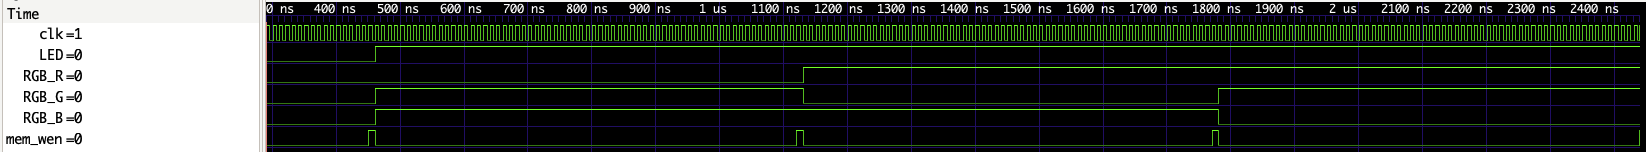
\includegraphics[width=\textwidth]{media/rgb_waveform}
    \caption{Waveform of the testbench for RGB LED. The waveform shows the RGB LEDs changing colors for a single loop.}
    \label{fig:rgb_waveform}
\end{figure}

Lastly, I wrote a simple assembly program to test the LED and RGB functionality of the RISC-V processor.
The program uses the \texttt{sw} instruction to store the RGB values in the memory address mapped to the RGB LEDs.
It uses \texttt{x7} register as a counter to create a delay between each color change by looping with branch and jump instructions.
As expected, the waveform in Figure~\ref{fig:rgb_waveform} shows the RGB LEDs changing colors in a loop.
